% 
% This message contains the LaTeX template for scribe notes
% in EE597.  You are free to use other means of producing
% your notes, but you are encouraged to use LaTeX: you will
% need to learn it some day.
% 
% Many thanks to Alistair Sinclair@cs.berkeley.edu for providing the basis for
% the first version of this template.
% 
% %************************************************************
%
% This is the LaTeX template file for lecture notes for EE596
% Pattern Recognition II: Introduction to Graphical Models.  When preparing 
% LaTeX notes for this class you must use this template.
%
% To familiarize yourself with this template, the body contains
% some examples of its use.  Look them over.  Then you can
% run LaTeX on this file.  After you have LaTeXed this file then
% you can look over the result either by printing it out with
% dvips or using xdvi.
%

\documentclass{article}
\usepackage{times,amsmath,amsthm,amsfonts,eucal,graphicx}
\usepackage{amssymb}
\usepackage[table]{xcolor}
\usepackage{tikz}

% This scribe template not only uses latex, but also
% the American Mathematical Society (AMS) latex macros.
% Detailed documentation on how to use them to produce good
% math formating can be obtained here: http://www.ams.org/tex/
% I've also placed a copy of the AMS-Latex documentation
% on the web page at:
%     http://www.ee.washington.edu/class/596/patrec/scribes/amsguide_2p.ps
% Latex documentation can be obtained from 
%
% Publications related to latex are listed here:
%     http://www.ams.org/tex/publications.html
%

\setlength{\oddsidemargin}{0.25 in}
\setlength{\evensidemargin}{-0.25 in}
\setlength{\topmargin}{-0.6 in}
\setlength{\textwidth}{6.5 in}
\setlength{\textheight}{8.5 in}
\setlength{\headsep}{0.75 in}
\setlength{\parindent}{0 in}
\setlength{\parskip}{0.1 in}

%
% The following commands set up the lecnum (lecture number)
% counter and make various numbering schemes work relative
% to the lecture number.
%
\newcounter{lecnum}
\renewcommand{\thepage}{\thelecnum-\arabic{page}}
\renewcommand{\thesection}{\thelecnum.\arabic{section}}
\renewcommand{\theequation}{\thelecnum.\arabic{equation}}
\renewcommand{\thefigure}{\thelecnum.\arabic{figure}}
\renewcommand{\thetable}{\thelecnum.\arabic{table}}

%
% A few symbols that we will be using often in this course.
\newcommand{\indep}{{\bot\negthickspace\negthickspace\bot}}
\newcommand{\notindep}{{\not\negthickspace\negthinspace{\bot\negthickspace\negthickspace\bot}}}
\newcommand{\definedtobe}{\stackrel{\Delta}{=}}
\renewcommand{\choose}[2]{{{#1}\atopwithdelims(){#2}}}
\newcommand{\argmax}[1]{{\hbox{$\underset{#1}{\mbox{argmax}}\;$}}}
\newcommand{\argmin}[1]{{\hbox{$\underset{#1}{\mbox{argmin}}\;$}}}

%
% The following macro is used to generate the header.
%
\newcommand{\lecture}[3]{
   \pagestyle{myheadings}
   \thispagestyle{plain}
   \newpage
   \setcounter{lecnum}{#1}
   \setcounter{page}{1}
   \noindent
   \begin{center}
   \framebox{
      \vbox{\vspace{2mm}
    \hbox to 6.58in { {\bf Depth First Learning
                        \hfill Wasserstein GAN} }
       \vspace{4mm}
       \hbox to 6.28in { {\Large \hfill Week #1:  #2 \hfill} }
       \vspace{2mm}
       \hbox to 6.28in { \hfill Scribed by: #3 }
      \vspace{2mm}}
   }
   \end{center}
   \markboth{Week #1: #2}{Week #1: #2}
   \vspace*{4mm}
}

%
% Convention for citations is authors' initials followed by the year.
% For example, to cite a paper by Leighton and Maggs you would type
% \cite{LM89}, and to cite a paper by Strassen you would type \cite{S69}.
% (To avoid bibliography problems, for now we redefine the \cite command.)
% Also commands that create a suitable format for the reference list.
\renewcommand{\cite}[1]{[#1]}
\def\beginrefs{\begin{list}%
        {[\arabic{equation}]}{\usecounter{equation}
         \setlength{\leftmargin}{2.0truecm}\setlength{\labelsep}{0.4truecm}%
         \setlength{\labelwidth}{1.6truecm}}}
\def\endrefs{\end{list}}
\def\bibentry#1{\item[\hbox{[#1]}]}

%Use this command for a figure; it puts a figure in wherever you want it.
%usage: \fig{NUMBER}{CAPTION}{.eps FILE TO INCLUDE}{WIDTH-IN-INCHES}
\newcommand{\fig}[4]{
			\begin{center}
	                \includegraphics[width=#4,clip=true]{#3} \\
			Figure \thelecnum.#1:~#2
			\end{center}
	}
% Use these for theorems, lemmas, proofs, etc.
\newtheorem{theorem}{Theorem}[lecnum]
\newtheorem{lemma}[theorem]{Lemma}
\newtheorem{proposition}[theorem]{Proposition}
\newtheorem{claim}[theorem]{Claim}
\newtheorem{corollary}[theorem]{Corollary}
\newtheorem{definition}[theorem]{Definition}
% \newenvironment{proof}{{\bf Proof:}}{\hfill\rule{2mm}{2mm}}

% **** IF YOU WANT TO DEFINE ADDITIONAL MACROS FOR YOURSELF, PUT THEM HERE:

\begin{document}
%FILL IN THE RIGHT INFO.
\lecture{1}{3 Feb, 2019}{Timothy Reeder, Julia Rozanova \& Sasha Naidoo}

\section{Overview}

The desired outcome for this week is that there is a good understanding of \textit{Kullback-Leibler Divergence}, maximising Likelihood, minimising Mean-Square error, and how they all relate to one another.

\section{Brief Feedback}

The course work for week 1 was very theoretical which confused the more practically inclined participants. In future it might be of benefit to have a broad discussion on the "bigger picture", maybe even a short practical approach. This would allow for a \textit{fill the gaps} learning approach rather than a \textit{build from the bottom up} approach, the latter being currently adopted. \newline
These concerns would be valuable to have on the collaborative Google document. This will alow for constructive conversations before the short time we have when meeting. 

\section{KL Divergence}

The weeks reading materials and exercises included the formula for \textit{KL Divergence} and \textit{R-KL Divergence}. A point of interest to someone first seeing these formulas is that: for the forward KL Divergence formula, the term that depends on the true distribution can be omitted - which is convenient since the true distribution is unknown. However, the Reverse KL Divergence formula depends on the true distribution. How then is this calculated?

This was left here to be taken up later.

An informal definition of KL Divergence is that it gives a distance/difference metric between two probability distributions.

The formula (1.1) was discussed and the simillarity it has with log-likelihood. P is your data and Q is your model. The formula can be re-written as (1.2) which shows you have the differential entropy of your data distribution and the expected value the model prediction. Which allows you to ignore the first term with a forward KL divergence. So when minimsing KL divergence, the goal is to maximise the remainf term (1.3). Which leaves us with the log likelihood of the model which is then maximum likelihood estimation.

\begin{center}
	\begin{flalign}
	D_{KL}(P||Q) &= \int_{\infty}^{-\infty}p(x)log(\frac{p(x)}{q(x)})dx \\
	D_{KL}(P||Q) &= \int_{\infty}^{-\infty}p(x)log(p(x))dx - \int_{\infty}^{-\infty}p(x)log(q(x))dx \\
	min(D_{KL}(P||Q)) &= - max(\int_{\infty}^{-\infty}p(x)log(q(x))dx)
	\end{flalign}
\end{center} 

\section{Side Notes}
\begin{itemize}
	\item When you have a probability density, you can have densities greater than 1. This is unintuitive since when considering a probability mass, it is between 0 and 1 always. However, this is not the case with a probability density function. This is when scaling occurs. Since if you scale the x-axis, the random variable will need to scale to fit. This could result in a probability density function being greater than 1, even though the mass will always remain between 0 and 1.
	\item The KL divergence of a distribution to itself is 0.
\end{itemize} 

\section{Equivalence between minimizing KL and maximizing likelihood}

\begin{itemize}
	\item It was deliberated upon for some time that we could say that
	\begin{equation}
	\frac{1}{N}\sum_{i=0}^N \log (q(x_i)) = \mathbb{E}_{x \sim p}[\log (q(x_i))].
	\end{equation}
	
	\item Martin pointed out that the above equality is a consequence of the ``Law of large numbers'' (for a large number of data points, the average value of $f(x)$ (in this case $(q(x_i))$) is a good approximation of its expectation).
	
	\item He also advised us that problems arise when you try and take the KL divergence between a discrete and a continuous distribution.
	
	\item It is actually a bit more	complicated: basically, one probability distribution should be absolutely continuous with respect to another if we wish to meaningfully take the KL divergence between them. There are certain requirements that need to be met, such as simultaneously assigning a 0 probability to sets of measure 0 (the details should
	be looked into more formally, if the reader is interested).
\end{itemize}

\section{Reverse KL divergence}

\begin{itemize}
	\item The formula for reverse KL divergence was inspected closely, and it was remarked that the
	\begin{equation}
	\mathbb{E}_{x \sim q_\theta}[\log (p(x))]
	\end{equation}
	term was a spanner in the works, as we do not have access to the ``true'' distribution $p(x)$ of the underlying	data.

	\item Martin asked a probing question: ``Can you think of any real-life examples where reverse KL is used to fit
	a model?''
	
	\item This isn’t really done, as this isn’t practically possible without an explicit p(x), which we wouldn’t have in such a context. However, reverse KL can be used in some situations: distillation problems, autoregressive models, parallel wavenet (where we have a good density model which is hard to sample from).
\end{itemize}

\section{Equivalence between minimising MSE and maximising likelihood}

\begin{itemize}
	\item It was suggested that a Gaussian distribution was a useful thing to assume, especially so as to avoid	assigning zero probability to any values that aren’t exactly some observed data point.
	
	\item Writing out the expression for the likelihood explicitly, $p(x|\theta)$ was shown to be proportional to an exponential function with a sum of square errors on the exponent. By monotonicity, we could maximise the likelihood by minimising the sum of square errors in this exponent, which is equivalent up to a constant factor to the MSE technique.
	
	\item The key observation was how, in this particular problem with the assumption of a Gaussian distribution,
	the following are equivalent:
	\begin{itemize}
		\item Maximising Likelihood
		\item Minimising the KL Divergence
		\item Minimising the Mean Square Error
	\end{itemize}
\end{itemize}

\section{Probability Distance Metrics} % Don't be this informal in your notes!

There are two classes of \textit{probability distance metrics}: F-divergences and Integral Probability Metrics (IPMs). Loosely, the F-divergences determine distance using division of two probability distributions, $\frac{P(x)}{Q(x)}$ and the IPMs use the difference, $P(x) - Q(x)$. There are various metrics that fall within each class. For F-divergences, we have the Kullback-Liebler (KL) divergence, Reverse-KL divergence and Jenson-Shannon Divergence (JSD). For the IPMS, we have the Wassterstein distance (which is used in the WGAN) and the Maximum Mean Discrepancy (MMD). The Total Variation (TV) metric overlaps between these two classes. These metrics are depicted in Figure~\ref{pdm}.

\begin{figure}[h]
	\begin{center}
		
		\begin{tikzpicture}[fill=blue!10,scale=2]
		% left hand
		%\scope
		%\clip (-2,-2) rectangle (2,2)
		%(1,0) circle (1);
		%\fill (0,0) circle (1);
		%\endscope
		% right hand
		%\scope
		%\clip (-2,-2) rectangle (2,2)
		%(0,0) circle (1);
		%\fill (1,0) circle (1);
		%\endscope
		% outline
		\draw (0,0) circle (1) (-0.3,1)  node [text=black,above] {F-div $\frac{P(x)}{Q(x)}$}
		(1,0) circle (1) (1.1,1)  node [text=black,above] {IPM $P(x) - Q(x)$}
		(0,0) circle (1) (-0.3,-0.8)  node [text=black,above] {KL Div}
		(0,0) circle (1) (-0.4,-0.2)  node [text=black,above] {R-KL Div}
		(0,0) circle (1) (-0.3,0.3)  node [text=black,above] {JSD}
		(0,0) circle (1) (0.5,-0.2)  node [text=black,above] {TV}
		(0,0) circle (1) (1.4,0.3)  node [text=black,above] {Wasserstein}
		(0,0) circle (1) (1.4,-0.3)  node [text=black,above] {MMD}
		;
		%(-2,-2) rectangle (3,2) noe [text=black,above] {$H$};
		\end{tikzpicture}
	\end{center}
	\caption{Classes of Probability Metrics.}
	\label{pdm}
\end{figure}

The different metrics of measuring distance between two probability distributions forms the main diversity for many GAN algorithms. The various GAN techniques take advantage of the different properties of each distance to suit the application.

\section{Maximum Likelihood}

When trying to model a dataset, we are trying to find the parameters, $\theta$, of a model that best represents the data. To do this, we take advantage of the relationship defined in Equation (1.1). For Maximum Likelihood Estimation, we are maximising the $p(x| \theta)$ in order to find the parameters $\theta$. By focusing only on maximising this probability distribution, this often leads to over-fitting. In order to address this issue, we typically include a form of regularisation which takes into account our prior belief of the parameters, $p(\theta)$. For example, L2-regularisation imposes a restriction that the parameters of the model are Guassian distributed, such that the model is penalised for having large valued parameters. 

\begin{center}
	\begin{flalign}
	p(\theta | x) & \propto p(x | \theta) & \\
	& = \frac{p(x | \theta)p(\theta)}{p(x)} \text{ (Bayes Rule)}
	\end{flalign}
\end{center}

Additionally, determining $p(x)$ can be very computationally challenging. In order to deal with this, it is possible to compute a point estimate of this distribution, which is called a \textit{MAP estimate}.

% **** THIS ENDS THE EXAMPLES. DON'T DELETE THE FOLLOWING LINE:

\end{document}


